\documentclass[conference]{IEEEtran}
\IEEEoverridecommandlockouts
\renewcommand\IEEEkeywordsname{Keywords}
% The preceding line is only needed to identify funding in the first footnote. If that is unneeded, please comment it out.
%for tables

\usepackage{booktabs}
\usepackage{multirow}
%end for tables
\usepackage{cite}
\usepackage{balance}

\usepackage{amsmath,amssymb,amsfonts} %Mathematical Symbol,Equation
\usepackage{algorithm}
\usepackage{hyperref}
\hypersetup{
    colorlinks=true,
    linkcolor=blue,
    filecolor=magenta,      
    urlcolor=cyan,
    citecolor=green,
    pdftitle={Password Shield},
    pdfpagemode=FullScreen,
    }
% \usepackage[linesnumbered,ruled]{algorithm2e}
%\usepackage[options ]{algorithm2e}
%\usepackage{algorithmic}
\usepackage{algpseudocode}
\usepackage{graphicx} %Adding picture \& figure
\usepackage{float} %Figure Alignment
\usepackage{textcomp} %Text formatting
\usepackage{eso-pic}
\usepackage{xcolor}
\usepackage{comment}
\usepackage{csquotes}
\def\BibTeX{{\rm B\kern-.05em{\sc i\kern-.025em b}\kern-.08em
    T\kern-.1667em\lower.7ex\hbox{E}\kern-.125emX}}
    
\makeatletter
%%%%%%%%%%%%%%%%%%%%%%%%%%%%%% User specified LaTeX commands.
% \def\ps@IEEEtitlepagestyle{%
%   \def\@oddfoot{\mycopyrightnotice}%
%   \def\@evenfoot{}%
% }
% \def\mycopyrightnotice{%
%  {\footnotesize 979-8-3503-5901-5/23/\$31.00  \textcopyright 2023 IEEE\hfill}% <--- Change here
%   \gdef\mycopyrightnotice{}% just in case
% }

\newcommand{\snippet}[1]{``\texttt{#1}''}



\usepackage{eso-pic}
\newcommand\AtPageUpperMyright[1]{\AtPageUpperLeft{%
 \put(\LenToUnit{0.5\paperwidth},\LenToUnit{-1cm}){%
     \parbox{0.5\textwidth}{\raggedleft\fontsize{9}{11}\selectfont #1}}%
 }}%
\newcommand{\conf}[1]{%
\AddToShipoutPictureBG*{%
\AtPageUpperMyright{#1}
}
}
%\hyphenation{op-tical net-works semi-conduc-tor}
\usepackage{fancyhdr}
%\usepackage[caption=false,font=footnotesize]{subfig}

% \renewcommand{\thispagestyle}[2]{} 


% \fancypagestyle{plain}{
%         \fancyhead{}
%         \fancyhead[C]{first page center header}
%         %\fancyfoot{}
%         %\fancyfoot[C]{first page center footer}
% }
% \pagestyle{fancy}
% \headheight 20pt
% \footskip 20pt
% \lhead{}
%\setcounter{page}{1}




\setlength {\marginparwidth }{2cm} 

\makeatletter
\def\footnoterule{\kern-3\p@
  \hrule \@width 2in \kern 2.6\p@} % the \hrule is .4pt high
\makeatother



\begin{document}


% Creating a custom header for the first page
\makeatletter

% Header settings

\title{Energy-Efficient IoT and Cloud Framework for Accurate and Scalable Hotel Occupancy Monitoring}

% Radar-IoT Fusion for Transparent Hotel Operations and Guest Monitoring.

%Authors
\author{\IEEEauthorblockN{Mahbubul Islam\IEEEauthorrefmark{1}, Md. Sahadat Hossain Sani\IEEEauthorrefmark{1}, Md. Mamun Hossain\IEEEauthorrefmark{1}, Md. Rakibul Hasan\IEEEauthorrefmark{1}, \& A B M Shawkat Ali\IEEEauthorrefmark{2}}

\IEEEauthorblockA{\textit{Department of Computer Science and Engineering}\\ 
\textit{Bangladesh University of Business and Technology, Dhaka, Bangladesh} \\
mahbubul2313@gmail.com\IEEEauthorrefmark{1},
sahadatsani@bubt.edu.bd\IEEEauthorrefmark{1},
mamunhasan.cs@gmail.com\IEEEauthorrefmark{1},\\
rakibhasan01316980149@gmail.com\IEEEauthorrefmark{1},
\& shawkat.ali@bubt.edu.bd\IEEEauthorrefmark{2} }}






\maketitle


% The paper headers and footers
\thispagestyle{fancyplain}
\fancyhf{}
\lhead{\fancyplain{}{11th IEEE International Conference on Sustainable Technology and Engineering\\02-04 December 2025, Washington University of Science and Technology,
United States of America}}
\lfoot{\fancyplain{}{979-8-3315-8316-3/25/\$31.00 ©2025 IEEE}}
\renewcommand{\headrulewidth}{0pt}

%%%%%%%%%%%%%%%%%%%%%%%%%%%%%%%%%%%%%%%%%%%%%%%%%%%%%%%%%%%%%%%%%%%%%%%%%%%%%%%%
\begin{abstract}
Efficient room occupancy monitoring is crucial for optimizing operations in the hospitality industry, yet traditional methods like manual reporting, camera-based systems, and passive infrared (PIR) sensors suffer from inaccuracies, privacy issues, and inability to detect stationary occupants. This paper introduces a cloud-integrated IoT solution that employs an ESP32 microcontroller interfaced with an HLK-LD2410B mmWave radar sensor to accurately detect both static and dynamic human presence. The system captures raw data via Universal Asynchronous Receiver/Transmitter (UART), processes it to determine occupancy status, and stores it locally using flash memory, while syncing with a Firebase Realtime Database for remote access. Energy efficiency is enhanced through deep sleep modes, with dynamic Wi-Fi provisioning via a captive portal and Over-the-Air (OTA) updates ensuring system adaptability. A Django-based web dashboard offers real-time occupancy updates, historical trends, and analytical visuals to support hotel management decisions. Tested over seven days across three hotel rooms with bi-minute sampling, the system achieved a 94.4\% detection accuracy, validated against manual observations, outperforming PIR-based alternatives. This scalable, privacy-focused framework holds promise for applications in smart homes, offices, healthcare facilities, and intelligent building management.

\end{abstract}


%\vspace{2mm}
\begin{IEEEkeywords}
\textcolor{black}{\textit{IoT \& Cloud, mmWave Radar, Energy Efficient, Cloud Integration, Occupancy Detection, Hospitality Management}}
\end{IEEEkeywords}

\section{Introduction}
\label{sec:Introduction}

Accurate room occupancy monitoring is a critical requirement in the hospitality industry, directly influencing operational decision-making, resource allocation, and revenue optimization~\cite{10421035}. Traditional approaches often rely on manual reporting by hotel staff, which is prone to human error, delayed updates, and in some cases, intentional misrepresentation~\cite{Mares2023}. These limitations reduce management efficiency and transparency, underscoring the need for automated and reliable monitoring systems that provide real-time insights regardless of location.

The rapid growth of the Internet of Things (IoT) has enabled the development of low-cost and energy-efficient monitoring frameworks that combine embedded devices with cloud-based services~\cite{https://doi.org/10.1155/2023/8571506}. Such systems have demonstrated success across domains such as smart homes, offices, and healthcare. However, within the hospitality sector, many existing solutions depend on camera-based surveillance or RFID key card logs. These methods either compromise guest privacy, demand costly infrastructure, or fail to provide continuous occupancy data. This gap motivates the design of a privacy-preserving, scalable, and transparent system that can deliver reliable real-time occupancy information.

In this paper, we propose an IoT-enabled hotel room monitoring system that leverages an ESP32 microcontroller integrated with the HLK-LD2410B human presence radar sensor for precise occupancy detection. Unlike PIR-based solutions, this radar sensor can identify both static and dynamic occupants, ensuring more reliable detection. Raw sensor data are captured via UART communication~\cite{10612928}, decoded, and processed to generate occupancy status and distance measurements. Data are stored locally in the ESP32’s SPIFFS file system and simultaneously synchronized with the Firebase Realtime Database, enabling remote accessibility. A Django-based web dashboard further provides hotel administrators with real-time visualization, historical usage trends, and analytical reports.

To ensure sustainability and long-term adaptability, the system incorporates multiple features: (i) a Wi-Fi Manager for flexible network configuration without hardcoded credentials, (ii) Over-the-Air (OTA) updates for remote firmware maintenance~\cite{10900824}, and (iii) deep sleep duty cycling to minimize energy consumption. These design choices make the proposed framework not only suitable for hotels but also extendable to smart buildings, office automation, healthcare facilities, classrooms, and industrial environments where occupancy-driven management is essential.

%%%%%%%%%review
Therefore, this study seeks to answer the following research question: \textit{“How can a radar-based IoT and cloud-integrated framework improve accuracy, scalability, and energy efficiency in hotel room occupancy monitoring compared to conventional PIR-based systems?”}
%%%%%%%%%%%
The main contributions of this paper are summarized as follows:
\begin{itemize}
    \item Development of a low-cost IoT-based hotel room occupancy detection system using radar sensing for both static and dynamic presence.
    \item Cloud-based storage and visualization through Firebase and a Django dashboard, enabling real-time and historical monitoring.
    \item Energy-efficient and sustainable operation using deep sleep, Wi-Fi Manager, and OTA-enabled remote maintenance.
    \item Demonstration of scalability across domains beyond hospitality, including smart homes, healthcare, and intelligent building systems.
\end{itemize}

The remainder of this paper is organized as follows: Section~\ref{sec:related-works} reviews related work and their limitations. Section~\ref{sec:Methodology} details the Methodology, including decoding, and additional features. Section~\ref{sec:analysis-results} presents performance evaluation and analysis. Finally, Section~\ref{sec:conclusion} concludes the paper with key findings, limitations, and directions for future research.

\section{Related Works}
\label{sec:related-works}

Automated occupancy monitoring has been widely investigated, with solutions ranging from simple motion sensors to advanced radar- and IoT-enabled frameworks. Early systems primarily relied on passive infrared (PIR) sensors integrated with microcontrollers. For instance, Leech et al.~\cite{leech2017pir} developed a real-time occupancy estimation approach using a single PIR sensor combined with Bayesian machine learning. Although privacy-friendly, PIR-based methods are limited to motion detection, cannot identify static occupants, and do not support end-to-end IoT pipelines.  

Radar-based techniques offer richer sensing capabilities, detecting fine-grained activities such as breathing and posture changes. Shen et al.\cite{shen2024radar} demonstrated a multi-radar system for human tracking and fall detection with high accuracy, though its focus was healthcare applications and it lacked energy-efficient design. Similarly, Cui and Dahnoun\cite{cui2021mmwave} employed FMCW mmWave radars for precise detection but required continuous operation, increasing system complexity and energy consumption. Furthermore, such works did not incorporate scalability features such as Over-the-Air (OTA) updates.  

Other studies explored indirect or environmental signals. Jin et al.\cite{jin2018env} proposed occupancy detection using airflow and temperature, showing potential for energy optimization but offering limited adaptability for heterogeneous environments. Pathri et al.\cite{pathri2024hostel} introduced an IoT-based hostel management framework integrating multiple sensors for energy efficiency and security, but it lacked fine-grained occupancy detection. Taryudi et al.~\cite{taryudi2018iot} developed an IoT-based integrated home security and monitoring system using PIR, fire, and environmental sensors, though the design primarily targeted household safety rather than scalable hospitality or enterprise applications.  

Survey contributions have also provided valuable insights. Akkaya et al.\cite{akkaya2015survey} reviewed IoT-based occupancy monitoring techniques, emphasizing the role of multi-modal data fusion while noting deployment and integration challenges. Singh and Shimi\cite{singh2018room} investigated IoT-based room automation with PIR and cloud connectivity, focusing on comfort and energy efficiency but lacking continuous occupancy detection capabilities.  

In contrast, our proposed system combines a low-cost HLK-LD2410B human presence radar with a full-stack IoT pipeline. Unlike expensive FMCW radar systems, the LD2410B achieves accurate detection of both motion and static presence at a significantly lower cost. By integrating deep sleep duty cycling for energy efficiency, OTA firmware updates for maintainability, and Firebase-based cloud synchronization for scalability, the proposed framework delivers a comprehensive, privacy-preserving, and extensible solution applicable not only to hospitality but also to smart homes, offices, healthcare facilities, and intelligent-building systems. The novelty of this work lies in leveraging the LD2410B radar within a cloud-integrated IoT architecture that achieves OTA resilience, adaptive energy management, and scalable multi-room deployment, capabilities not demonstrated in prior LD2410B-based studies. A comparative summary of prior approaches and the proposed framework is presented in Table~\ref{tab:related-comparison}, highlighting the differences in detection capability, privacy, energy efficiency, and scalability.


% In contrast, our proposed system combines the low-cost HLK-LD2410B human presence radar with a full-stack IoT pipeline. Unlike expensive FMCW radar systems, the LD2410B achieves accurate detection of both motion and static presence at significantly lower cost. By integrating deep sleep duty cycling for energy efficiency, OTA firmware updates for maintainability, and Firebase-based cloud synchronization for scalability, the proposed framework delivers a comprehensive, privacy-preserving, and extensible solution applicable not only to hospitality but also to smart homes, offices, healthcare facilities, and intelligent building systems. A comparative summary of prior approaches and the proposed framework is presented in Table~\ref{tab:related-comparison}, highlighting differences in detection capability, privacy, energy efficiency, and scalability.  

\begin{table*}[htbp]
\centering
\caption{Comparison of Occupancy Monitoring Approaches}
\label{tab:related-comparison}
\begin{tabular}{|p{3cm}|p{3.2cm}|p{2.8cm}|p{3.2cm}|p{3.2cm}|}
\hline
\textbf{Approach} & \textbf{Detection Capability} & \textbf{Privacy} & \textbf{Energy Efficiency} & \textbf{Scalability / Cloud Support} \\ \hline

PIR-based 
(e.g.,~\cite{leech2017pir}, \cite{singh2018room}) 
& Motion only, no static detection 
& High (no images collected) 
& High (low power sensors) 
& Limited (no end-to-end IoT pipeline) \\ \hline

Radar-based FMCW 
(e.g.,~\cite{cui2021mmwave}, \cite{shen2024radar}) 
& Motion + fine-grained presence (e.g., breathing, posture) 
& High 
& Low (continuous high-power operation) 
& Limited (no OTA/cloud integration) \\ \hline

Environmental sensing 
(e.g.,~\cite{jin2018env}) 
& Indirect inference (airflow, temperature, CO\textsubscript{2}) 
& High 
& Medium (depends on number of sensors) 
& Low (poor adaptability and integration) \\ \hline

IoT multi-sensor 
(e.g.,~\cite{pathri2024hostel}, \cite{taryudi2018iot}) 
& Motion + environmental events (PIR, fire, temperature) 
& Medium (some personal data) 
& Medium (varies with sensor set) 
& Moderate (basic IoT integration, limited scalability) \\ \hline

\textbf{Proposed System} 
& Motion + static presence (LD2410B radar) 
& High (privacy-preserving, no camera) 
& High (deep sleep duty cycling on ESP32) 
& High (Firebase cloud sync + OTA updates) \\ \hline

\end{tabular}
\end{table*}


% \iffalse
% \begin{table}[htbp]
% \centering
% \hspace*{-2.5cm}
% \caption{Previous research works in terms of used techniques \& focused methods, and possible research gaps}
% \label{research work}
% \resizebox{0.5\textwidth}{!}{
% \begin{tabular}{|p{1.4cm}|p{1.1cm}|p{2.8cm}|p{2.2cm}|}
% \hline
% \textbf{Category} &
%   \textbf{Reference} &
%   \textbf{Techniques \& Methods} &
%   \textbf{Challenges/ Research Gaps} \\ \hline


%%%%%%%%%%%%%%%%%%%%%%%%%%%%%%%%%%%%%%%%%%%%%%%
\section{Methodology}
\label{sec:Methodology}
%\subsection{\textbf{System Overview}}
The implementation of the proposed hotel monitoring system integrates both hardware and software components to achieve reliable and automated room occupancy detection. The ESP32 microcontroller acts as the central unit, interfacing with the HLK-LD2410B radar sensor for presence detection, while also handling data storage, wireless communication, and remote update management. The overall architecture is designed to ensure accuracy, efficiency, and scalability. The major implementation aspects are discussed in the following subsections.

The overall methodological architecture of the system, given in figure \ref{fig:overallMethodology}, defines a structured workflow for continuous occupancy monitoring. Initially, the ESP32 wakes from deep sleep at predefined intervals and activates the radar sensor to capture human presence data. The raw hexadecimal data from the sensor is decoded into occupancy status and distance measurements. The processed information is simultaneously logged in the local SPIFFS flash memory and transmitted to the Firebase Realtime Database for remote access. Wi-Fi Manager ensures dynamic network provisioning, while OTA enables seamless firmware updates\cite{10376259, sadman2023password}. The system operation is visualized through a Django-based dashboard, displaying real-time room status, historical trends, and graphical analytics. This methodology ensures a scalable, energy-efficient, and reliable framework suitable for hotels as well as broader applications such as smart homes, offices, and intelligent buildings.

\begin{figure}[htbp]
    \centering
    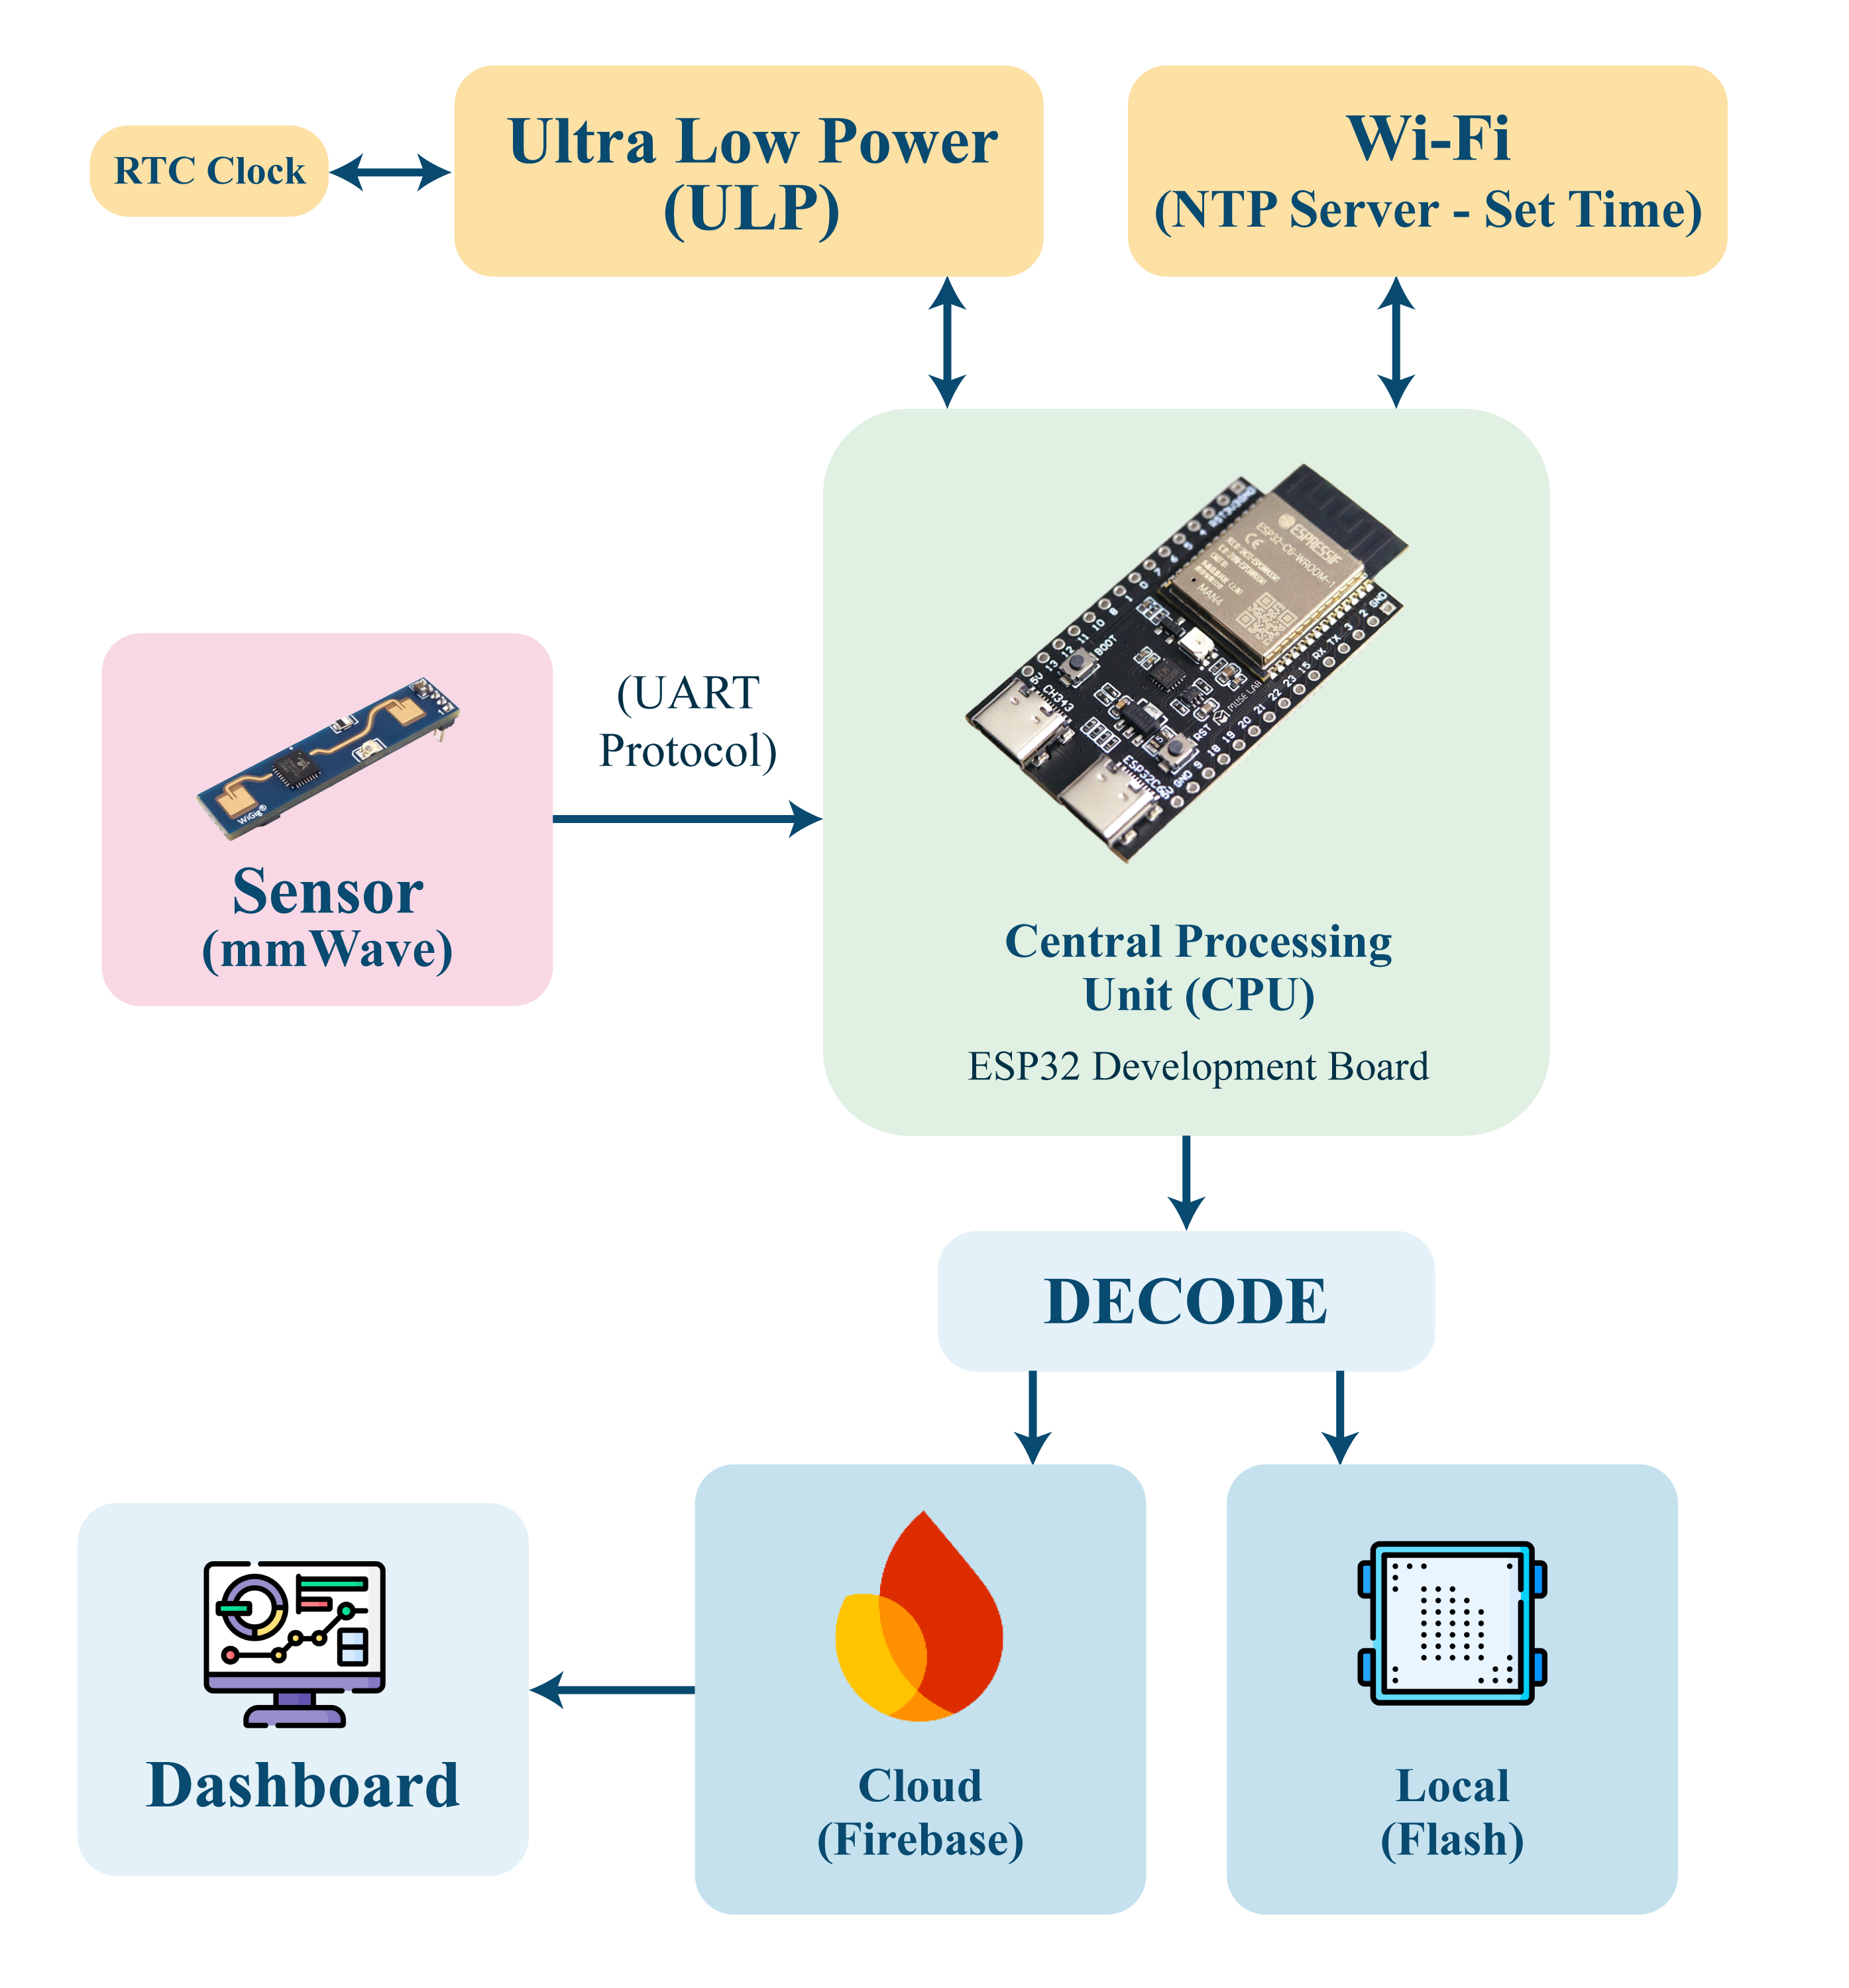
\includegraphics[width=0.8\linewidth]{Figures/methodology.png}
    \caption{Methodological Architecture}
    \label{fig:overallMethodology}
\end{figure}



\subsection{Decode}
The HLK-LD2410B radar sensor communicates via UART, transmitting raw hexadecimal data frames containing presence flags, distance measurements, and signal energy. The ESP32 parses these frames by validating the header, checksum, and payload length. Extracted values are processed to determine occupancy and distance metrics, while corrupted frames are discarded to reduce false positives. As shown in Fig. \ref{fig:frequencyDecoding}, this decoding module establishes reliable sensor–microcontroller communication, forming the foundation for accurate occupancy detection within the proposed monitoring system. 

\begin{figure}[htbp]
    \centering
    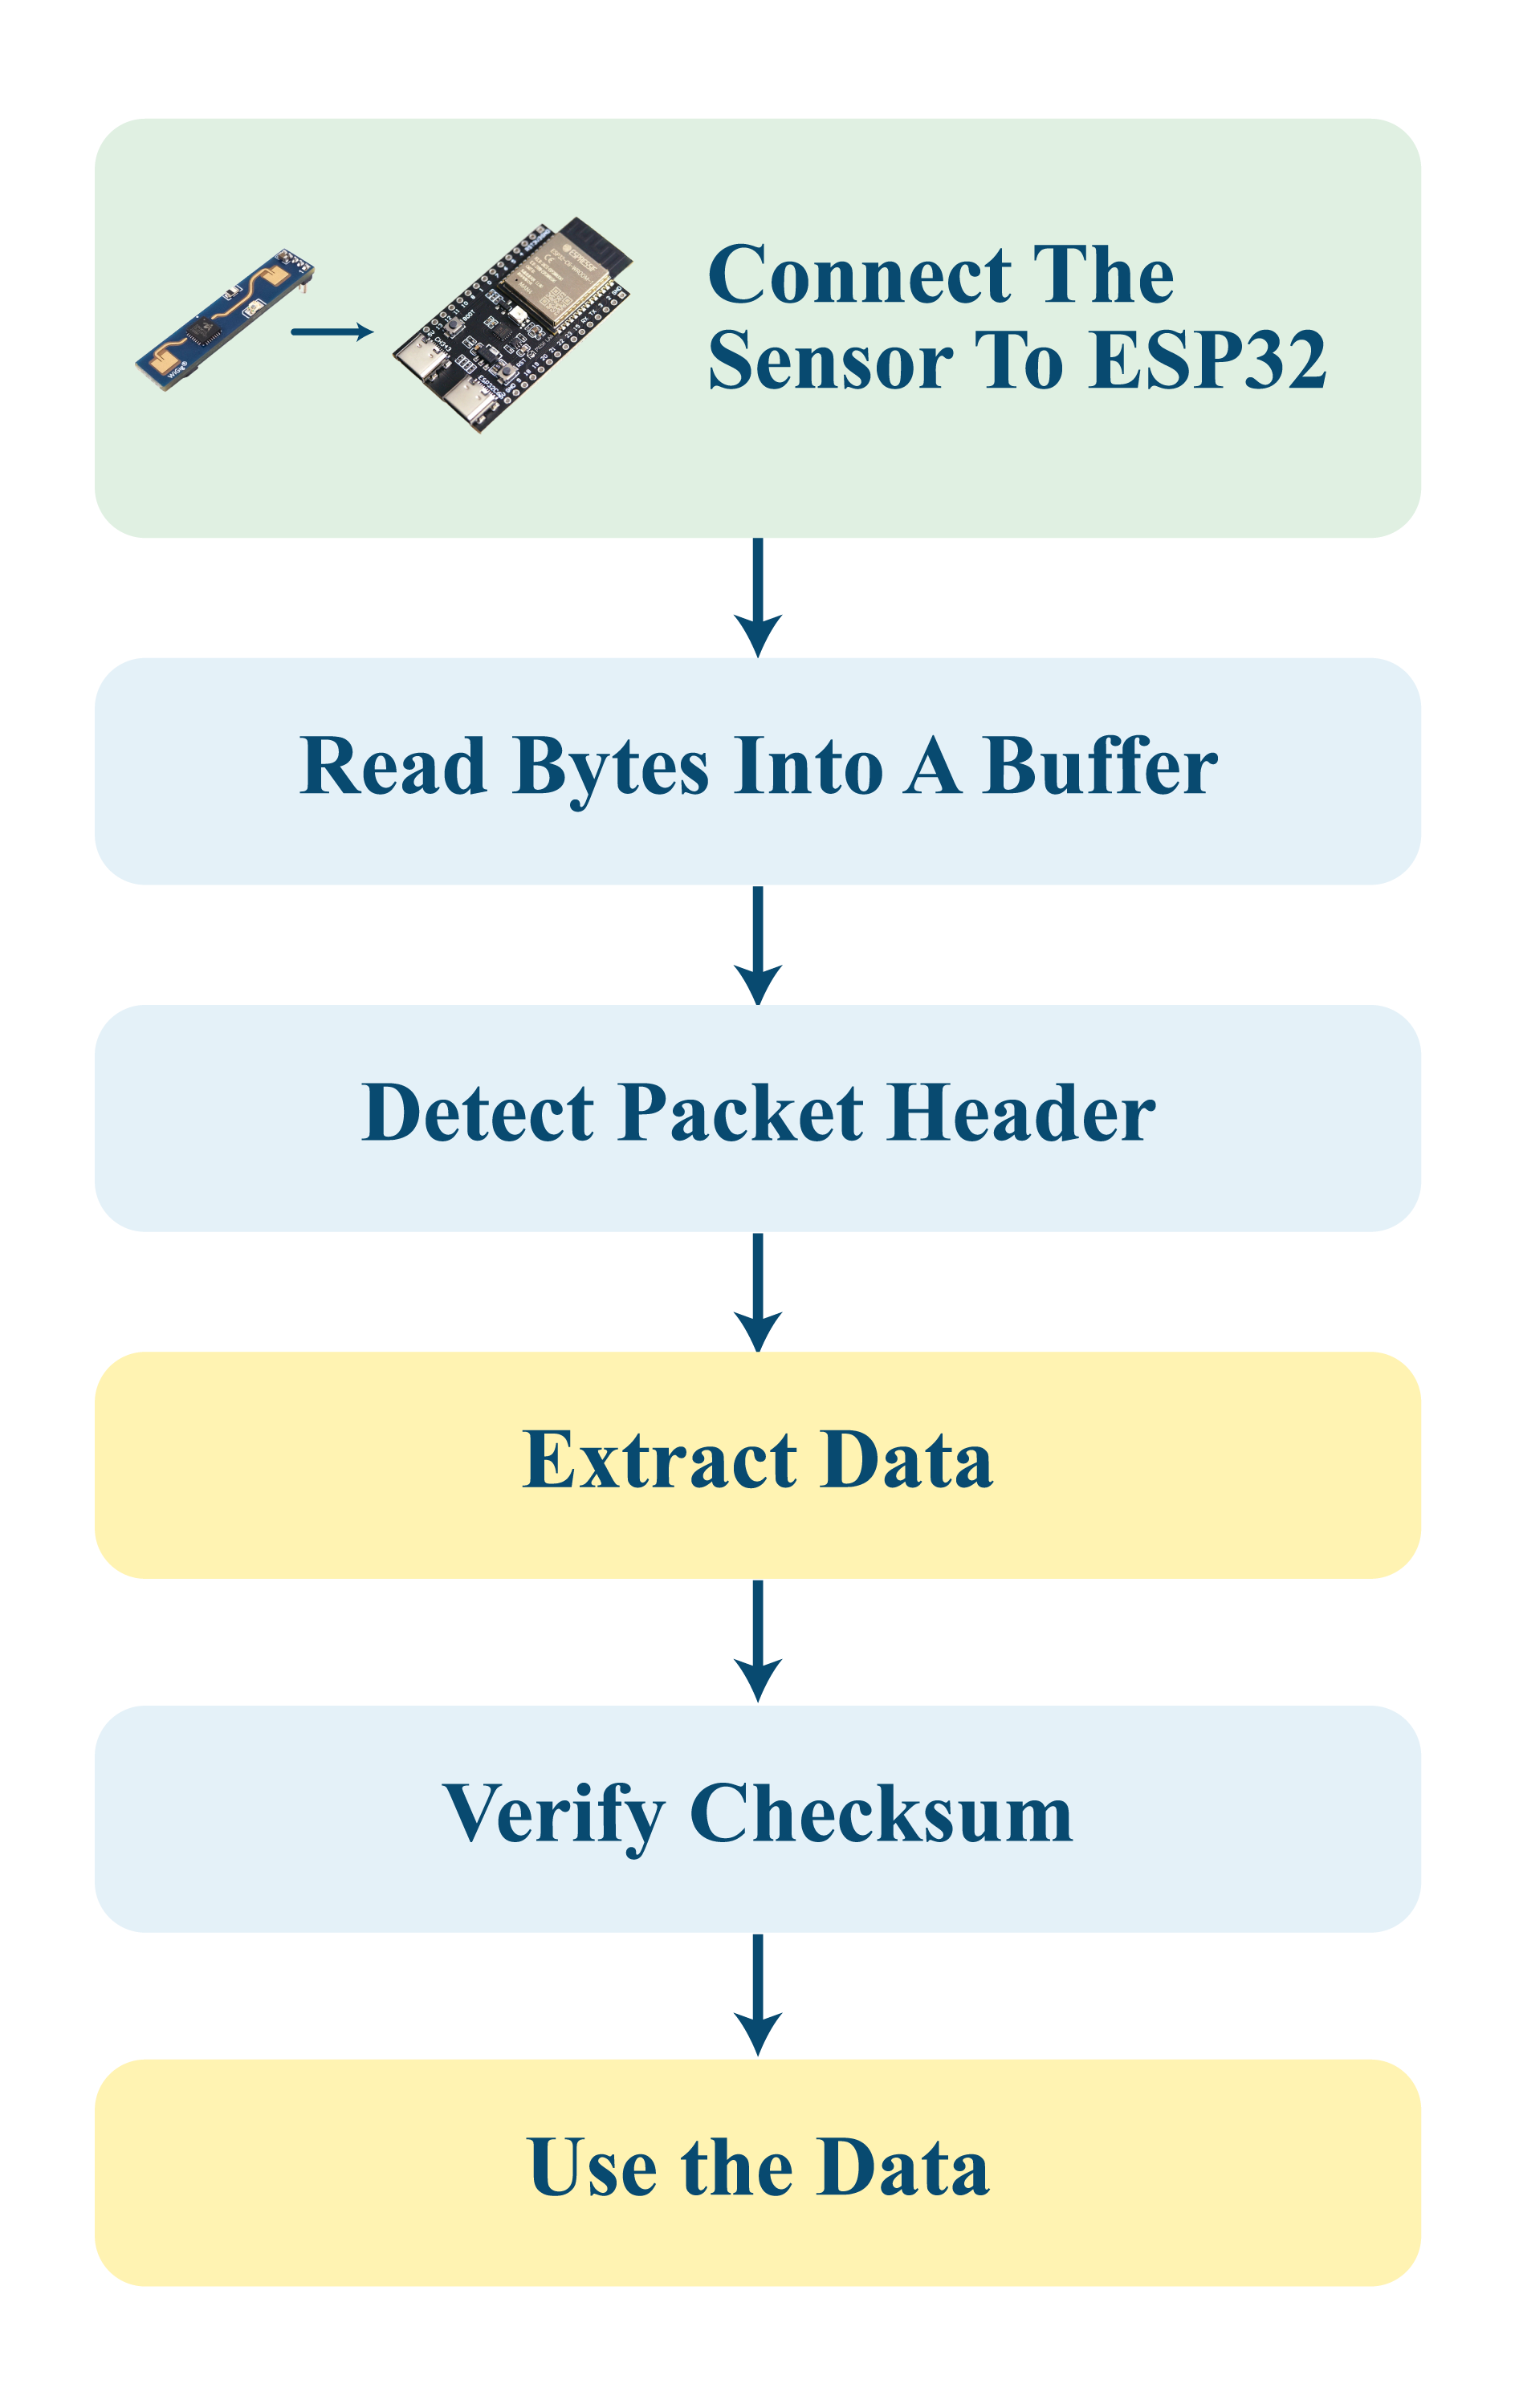
\includegraphics[width=0.6\linewidth]{Figures/decode.png}
    \caption{Frequency Decoding}
    \label{fig:frequencyDecoding}
\end{figure}

\subsection{Deep Sleep}
The ESP32 utilizes deep sleep mode to significantly reduce power consumption \cite{amslaurea31250}. After completing data collection and transmission, the device enters a low-power state and awakens periodically through the RTC timer \cite{10823195, hasan2024marvin}. This cycle enables long-term operation while still providing near real-time monitoring. As shown in Fig. \ref{fig:deepSleep}, the deep sleep mechanism ensures energy efficiency by balancing data accuracy with sustainable power usage, making the system suitable for continuous deployment in hotel environments.

\begin{figure}[htbp]
    \centering
    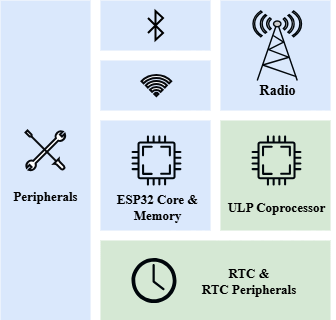
\includegraphics[width=1\linewidth]{Figures/deeps.png}
    \caption{Deep Sleep}
    \label{fig:deepSleep}
\end{figure}

\subsection{Wi-Fi Manager}
Wi-Fi Manager provides dynamic configuration for network connectivity without requiring hardcoded credentials. During initial setup, the ESP32 launches an Access Point and captive portal where hotel staff can input Wi-Fi credentials. These details are securely stored in non-volatile memory, allowing automatic reconnections during subsequent sessions. As shown in Fig. \ref{fig:WifiManager}, this feature simplifies deployment and enhances scalability, enabling flexible integration of the monitoring system across multiple hotel rooms.

\begin{figure}[htbp]
    \centering
    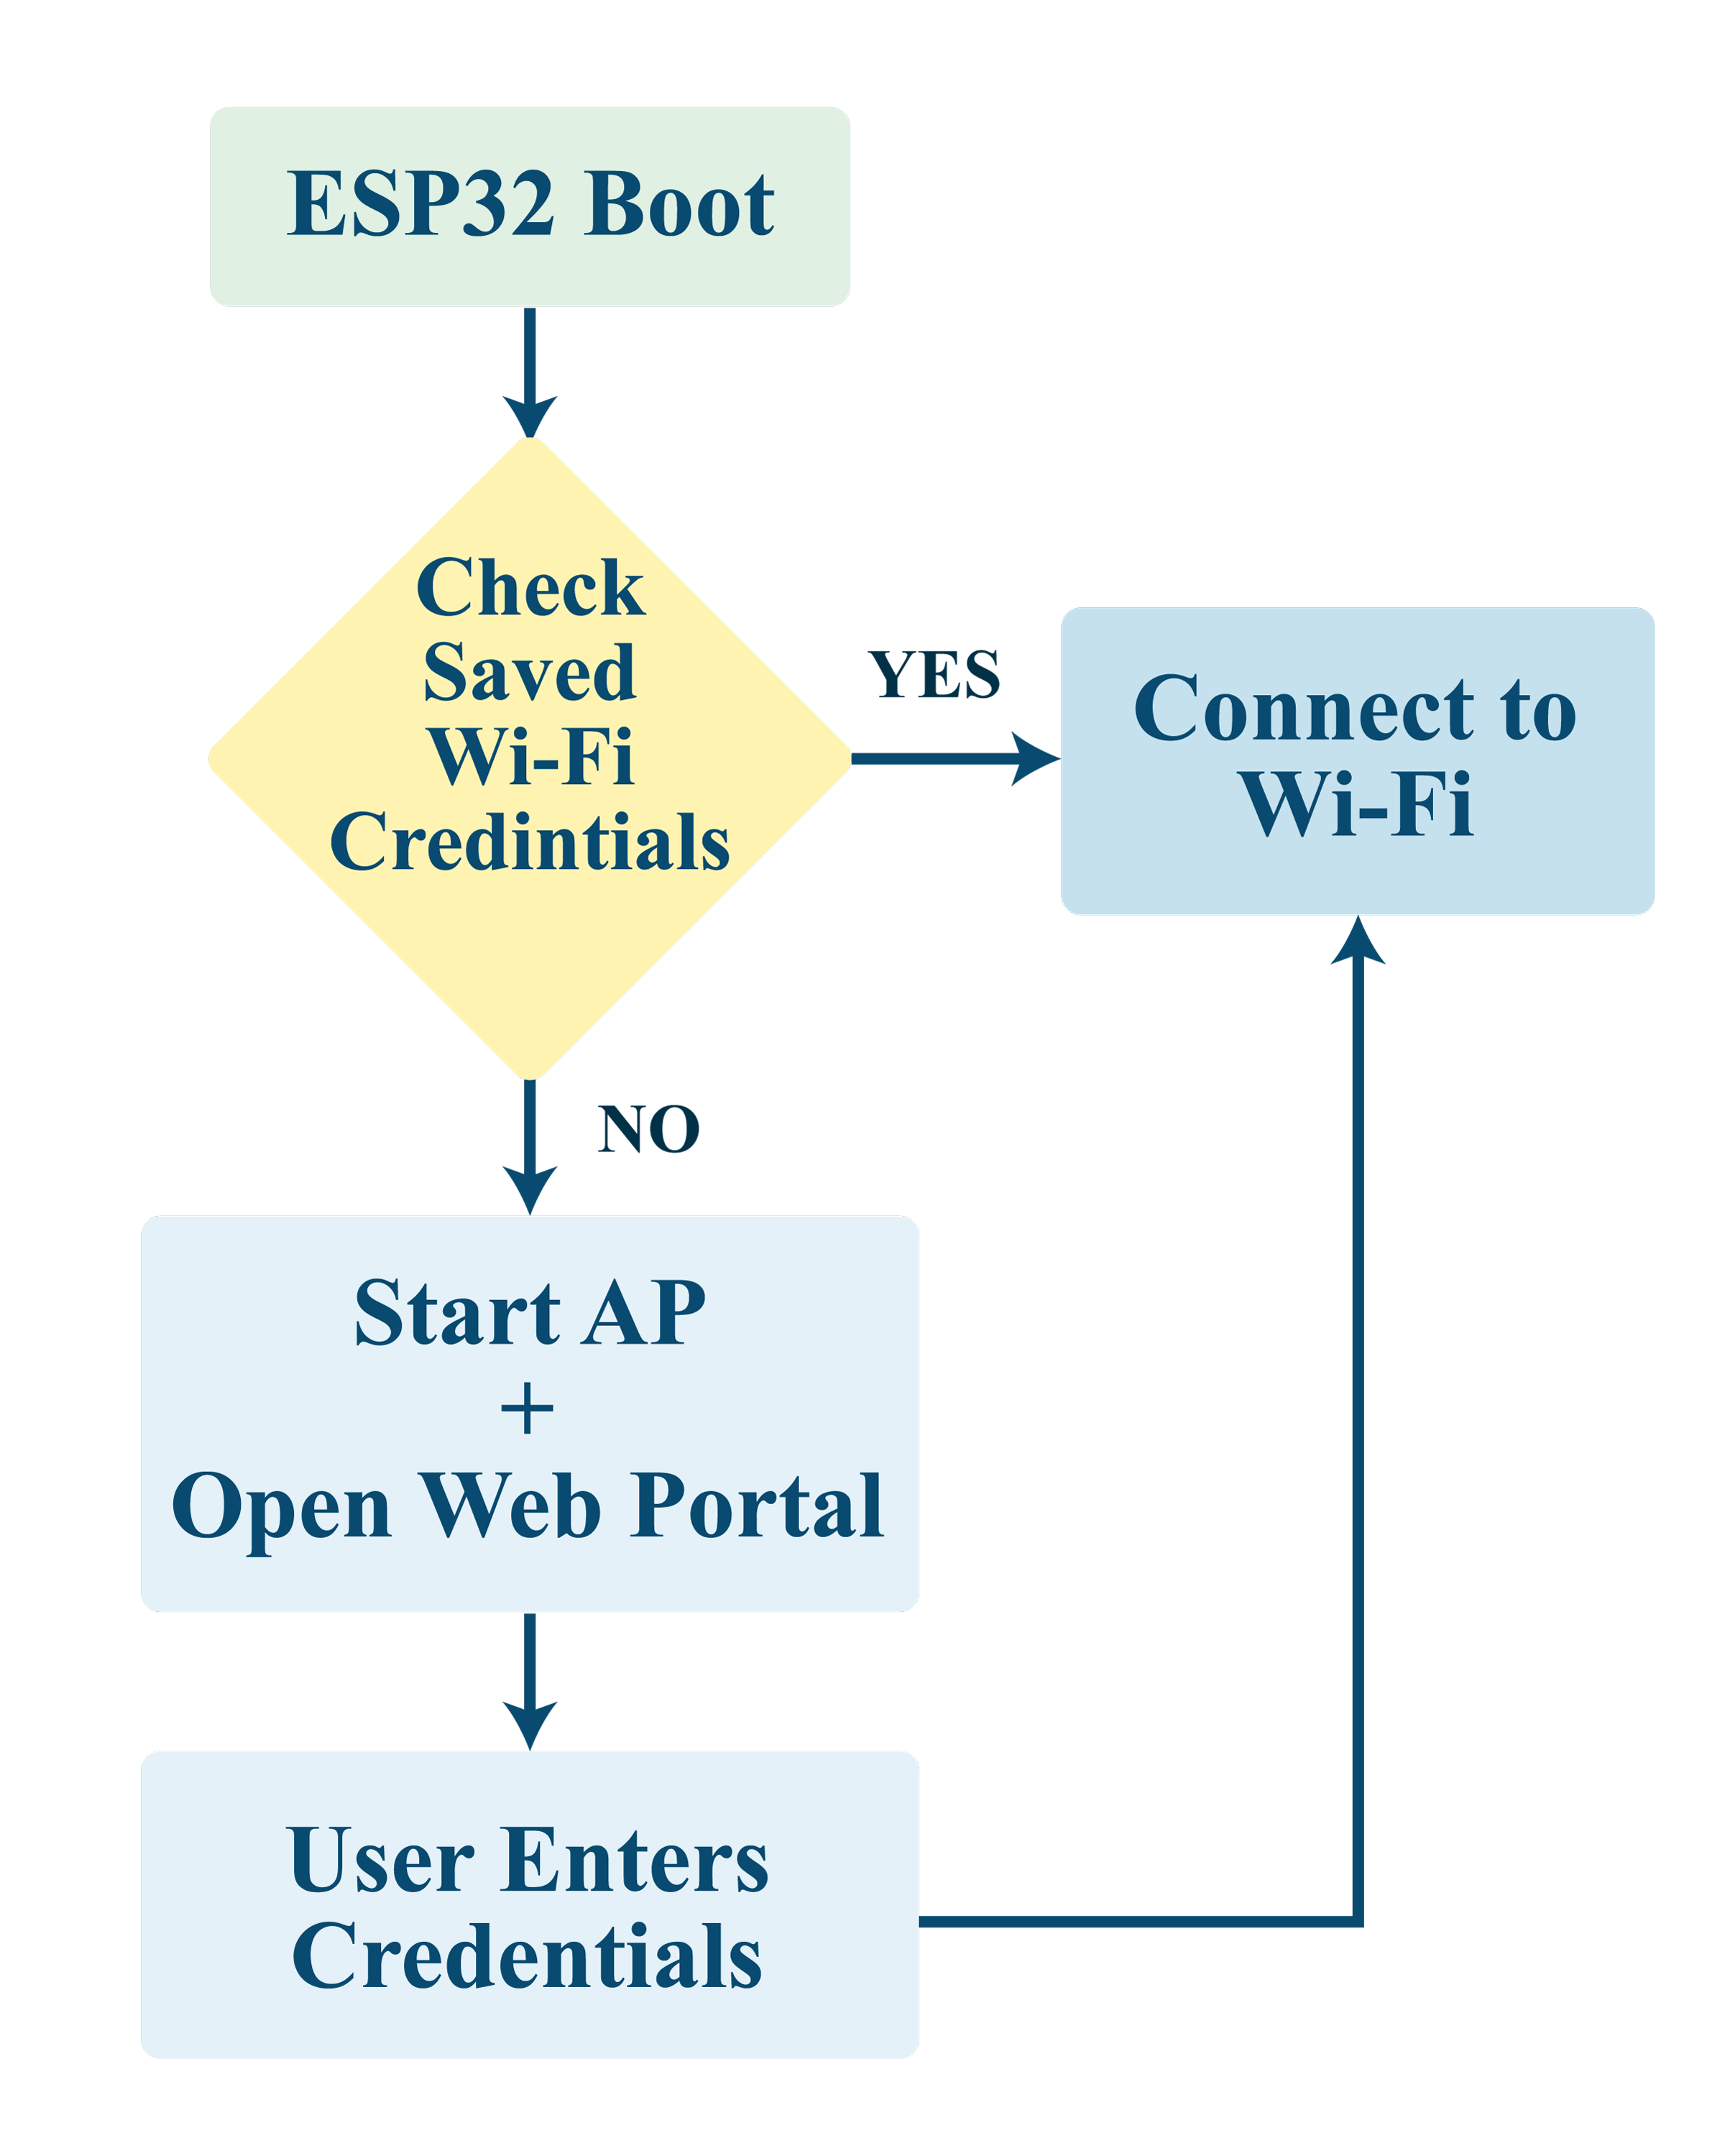
\includegraphics[width=0.6\linewidth]{Figures/wifi.png}
    \caption{Wifi manager}
    \label{fig:WifiManager}
\end{figure}

\subsection{Over The Air (OTA)}
Over-the-Air (OTA) updates enable remote firmware maintenance by allowing the ESP32 to securely download, validate, and install new software versions. In the event of an installation failure, the device automatically reverts to the previous stable firmware to ensure uninterrupted operation. As shown in Fig. \ref{fig:ota}, the OTA mechanism enhances system adaptability and maintainability, enabling continuous improvement of the occupancy monitoring framework without requiring on-site technical intervention.
\begin{figure}[htbp]
    \centering
    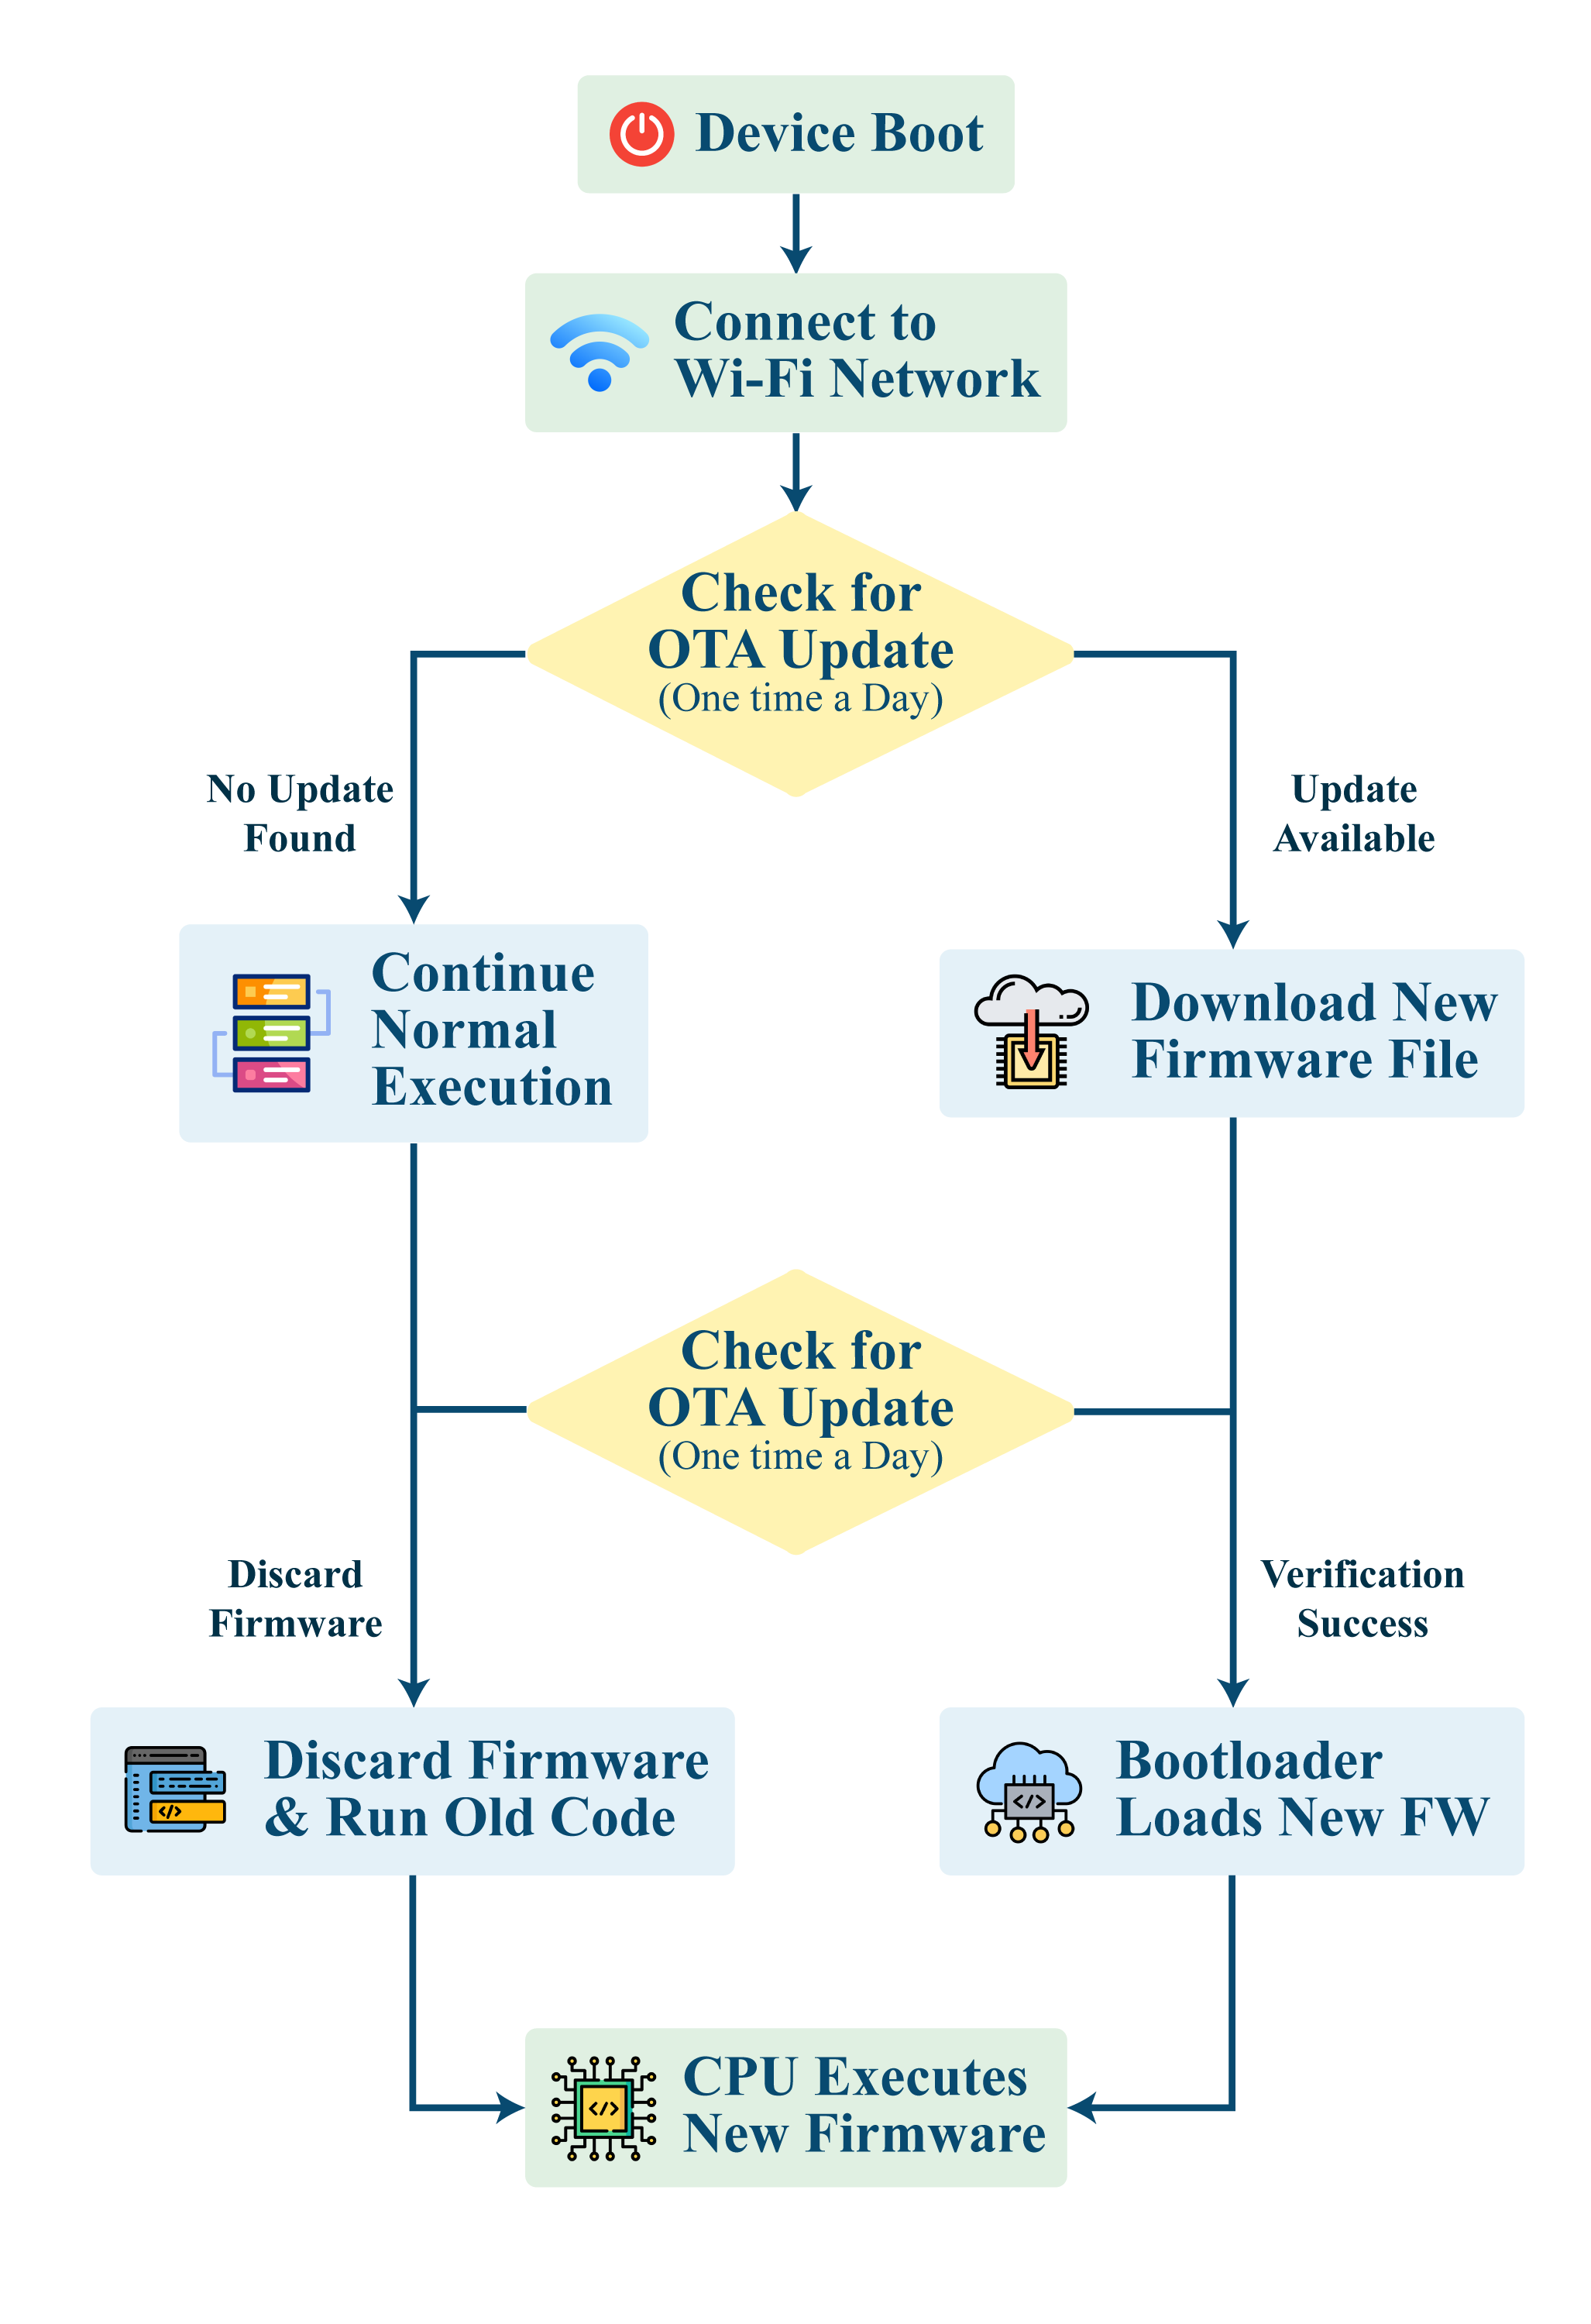
\includegraphics[width=1\linewidth]{Figures/ota.png}
    \caption{Over The Air (OTA)}
    \label{fig:ota}
\end{figure}

\subsection{Flash}
Local persistence is implemented using SPIFFS to store occupancy data in structured date-based CSV files\cite{10754923}. This ensures reliable logging in case of temporary network issues, allowing backlogged entries to be synchronized with the cloud once connectivity is restored. Data retention policies maintain recent records to prevent flash overflow.

\subsection{Web Application}
\label{subsec:web-app}

A Django-based web application was developed to provide hotel administrators with a user-friendly interface for monitoring room occupancy. The dashboard displays real-time status updates synchronized from the Firebase Realtime Database, while also allowing for historical analysis through graphical charts and trend visualizations. Data can be filtered by room, date, and occupancy frequency, supporting operational decision-making and resource allocation.

\begin{figure}[htbp]
    \centering
    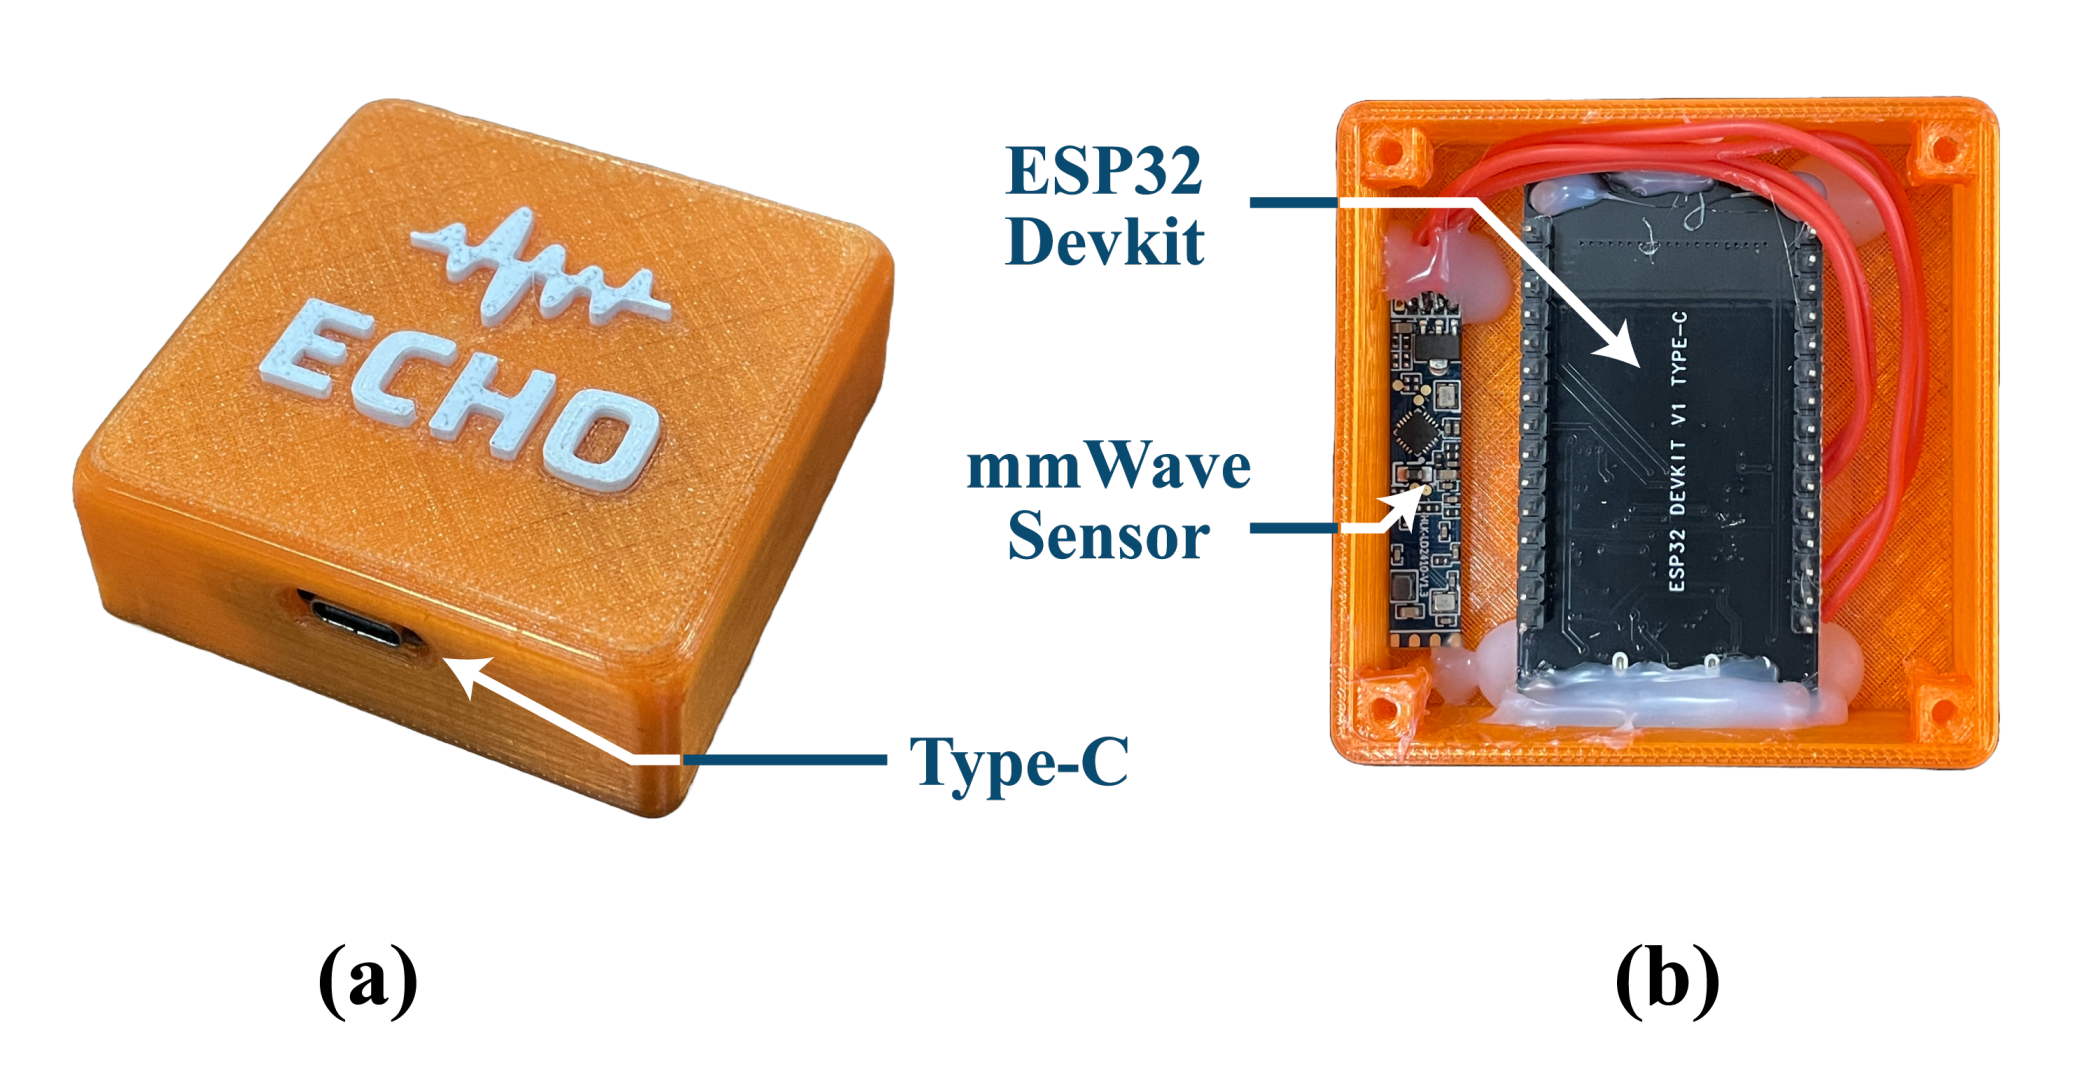
\includegraphics[width=1\linewidth]{Figures/view.png}
    \caption{Hardware architecture}
    \label{fig:ECHOhardware}
\end{figure}


\begin{figure}[htbp]
    \centering
    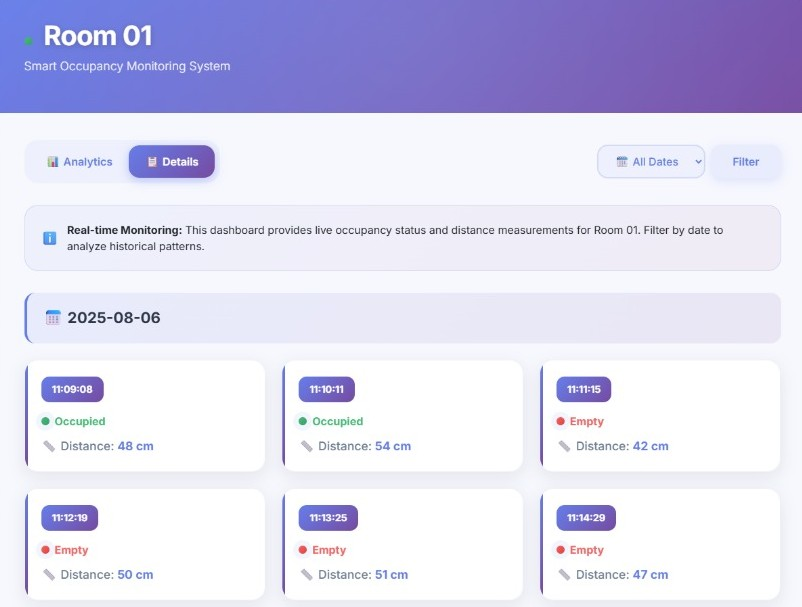
\includegraphics[width=1\linewidth]{Figures/web.jpeg}
    \caption{Web view}
    \label{fig:webdashboard1}
\end{figure}

\begin{figure}[htbp]
    \centering
    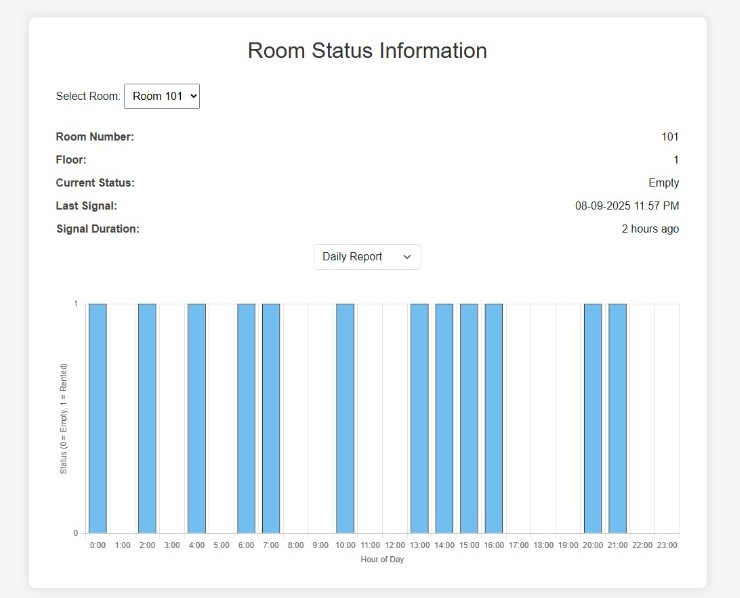
\includegraphics[width=1\linewidth]{Figures/daily.jpeg}
    \caption{Daily web view}
    \label{fig:webd}
\end{figure}
\begin{figure}[htbp]
    \centering
    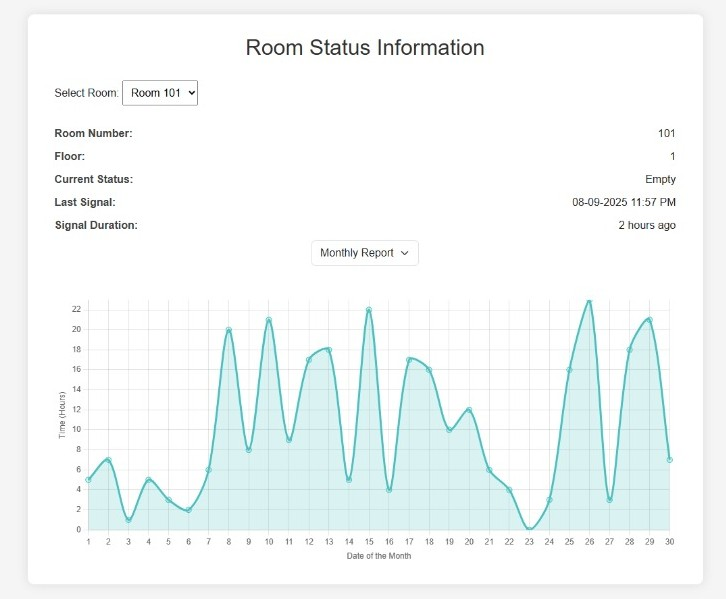
\includegraphics[width=1\linewidth]{Figures/monthly.jpeg}
    \caption{Monthly web view}
    \label{fig:webm}
\end{figure}

\section{Implementation \& Result Analysis}
\label{sec:analysis-results}

The room occupancy monitoring system, named ECHO, was implemented using an ESP32 microcontroller and an HLK-LD2410B sensor. The implementation integrates the functionalities described in the methodology, including data decoding, deep sleep mode, Wi-Fi manager, over-the-air (OTA) updates, and flash memory operations. To complete the prototype, a custom enclosure was designed and fabricated using a 3D printer. The final prototype of ECHO is shown in Fig. \ref{fig:ECHOhardware}.
We also make a Django-based web application for real-time monitoring. As shown in Fig. \ref{fig:webdashboard1}, the real-time dashboard provides immediate updates of room occupancy, enabling hotel managers to remotely track availability and reduce dependence on manual staff reporting. Fig. \ref{fig:webd}, illustrates the daily view, which highlights occupancy fluctuations within a 24-hour cycle and helps optimize housekeeping schedules and staff allocation. Finally, Fig. \ref{fig:webm}, presents the monthly trend analysis, allowing administrators to identify seasonal demand patterns, forecast room usage, and optimize energy consumption across facilities. Together, these views ensure that hotel owners, even when remote, can transparently access live and historical occupancy data, thereby improving efficiency, operational transparency, and long-term decision making.

The room occupancy monitoring system was deployed in three hotel rooms and evaluated continuously for a period of seven days. Sensor readings were taken every two minutes, resulting in 30 values per hour, 720 values per day, and a total of 5,040 values per room across the 7-day experiment. In total, the system generated 15,120 occupancy records across the three rooms, which were cross-verified with manual ground truth observations.

Out of a total of 15,120 occupancy events, the system correctly identified 14,280 events, resulting in an overall detection accuracy of 94.4\%. The majority of misclassifications were false negatives, while minor inaccuracies were also observed due to environmental and operational factors, including variations in lighting conditions, electromagnetic interference from adjacent rooms, and frequency overlaps from nearby electronic devices, which occasionally affected sensor readings.
A detailed summary of system performance for each room is presented in Table \ref{tab:occupancy_accuracy}. The system maintained consistent accuracy above 94.4\% across all three rooms.


% \begin{figure}[htbp]
%     \centering
%     \includegraphics[width=1\linewidth]{Figures/occupancy events.png}
%     \caption{Occupancy events frequency curve}
%     \label{fig:frequencycurve}
% \end{figure}


\begin{table}[htbp]
    \centering
    \caption{Summary of occupancy detection accuracy across three hotel rooms}
    \label{tab:occupancy_accuracy}
    \begin{tabular}{|c|c|c|c|}
        \hline
        \textbf{Trial} & \textbf{Total Events} & \textbf{Correctly Detected} & \textbf{Accuracy (\%)} \\
        \hline
        Room 1 & 5,040 & 4,763 & 94.5 \\
        Room 2 & 5,040 & 4,752 & 94.3 \\
        Room 3 & 5,040 & 4,765 & 94.6 \\
        \hline
        \textbf{Total} & \textbf{15,120} & \textbf{14,280} & \textbf{94.4} \\
        \hline
    \end{tabular}
    




    
\end{table}






% \begin{table}[htbp]
% \centering
% \caption{Argon2 Timings}
% \label{tab:Argon2-Table}
% \resizebox{0.5\textwidth}{!}{
% \begin{tabular}{|c|c|c|c|c|c|}
% \hline
% \textbf{Test} &
%   \textbf{\begin{tabular}[c]{@{}c@{}}Hash\\ Length\end{tabular}} &
%   \textbf{\begin{tabular}[c]{@{}c@{}}Memory \\ Cost\\ (KiB)\end{tabular}} &
%   \textbf{Parallelism} &
%   \textbf{\begin{tabular}[c]{@{}c@{}}Time \\ Cost\end{tabular}} &
%   \textbf{\begin{tabular}[c]{@{}c@{}}Per \\ Password\\ Verification\end{tabular}} \\ \hline
% 1                                                & 32 bytes & 2097152 & 4 threads & 1 iterations & 826.5 ms \\ \hline
% 2                                                  & 32 bytes & 65536   & 4 threads & 3 iterations & 55.2 ms  \\ \hline
% 3                                                             & 16 bytes & 102400  & 8 threads & 2 iterations & 61.6 ms  \\ \hline
% 4                                                     & 32 bytes & 244141  & 4 threads & 3 iterations & 211.6 ms \\ \hline
% \begin{tabular}[c]{@{}c@{}}5$^{\mathrm{*}}$ \end{tabular} & 32 bytes & 488281  & 4 threads & 3 iterations & 380.7 ms \\ \hline

% \multicolumn{6}{l}{$^{\mathrm{*}}$Default Argon2 Hashing Profile}
% \end{tabular}
% }
% \end{table}


\section{Conclusion}
\label{sec:conclusion}
The IoT-based Hotel Monitoring System effectively automates room occupancy detection using the ESP32 microcontroller and HLK-LD2410B radar sensor, combining local data processing, SPIFFS storage, cloud synchronization via Firebase, and visualization through a Django dashboard. It delivers accurate, real-time monitoring while optimizing energy efficiency through deep sleep and providing flexible deployment with Wi-Fi Manager and OTA updates. The system improves transparency, reduces operational errors, and supports data-driven decision-making for hotel administrators.

\section{Limitations \& Future Work}
\label{sec:limitation}
Although the proposed system achieves high accuracy and energy efficiency, several limitations remain. First, the framework depends on stable Wi-Fi connectivity for real-time cloud updates, which may cause delays during network outages. Additionally, the ESP32’s limited processing power and memory restrict complex signal processing and edge analytics. However, the seven-day deployment period provides only short-term validation and may not reflect long-term environmental variations. Finally, the radar sensor can also be affected by interference from nearby electronic devices or adjacent radars.
% Despite its capabilities, the system faces challenges such as reliance on network connectivity, limited on-device storage, and hardware constraints of the ESP32. 

While the system ensures privacy, future work should strengthen cloud data security and access control to support large-scale deployment. Additionally, future improvements could include multi-room integration with centralized dashboards, predictive analytics using machine learning to optimize occupancy and energy usage, sensor fusion for enhanced detection accuracy, mobile app support for real-time alerts, edge computing to reduce cloud dependency, and advanced security features including encrypted data transmission and user access control. These enhancements will expand the system’s scalability, intelligence, and applicability to broader domains such as smart homes, offices, healthcare facilities, and intelligent building management.
\balance
\bibliographystyle{IEEEtran}
\bibliography{ref}


\end{document}